\section{Experiments}
\label{sec:exp}

\begin{figure}[t]
\begin{tabular}{cc}
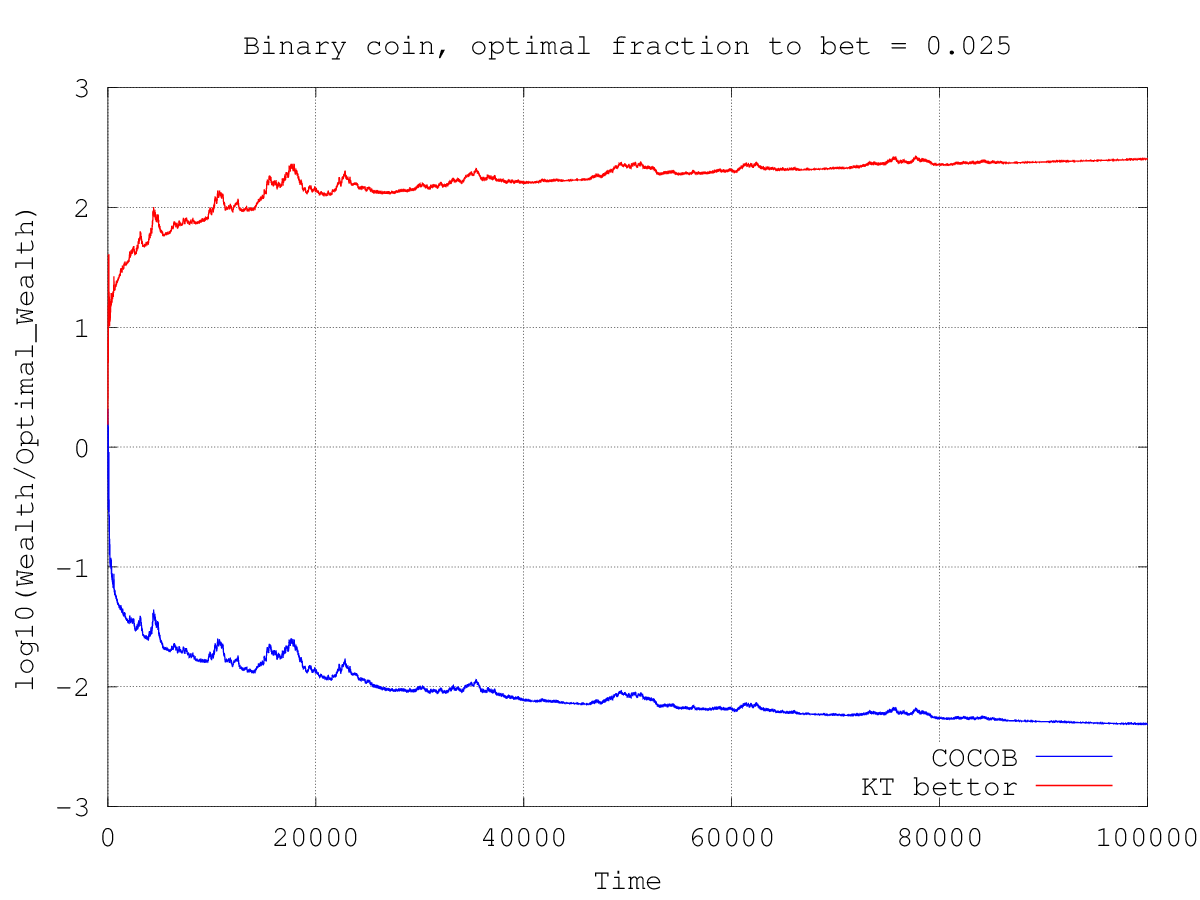
\includegraphics[width=0.45\linewidth]{code/binary_coin.png} &
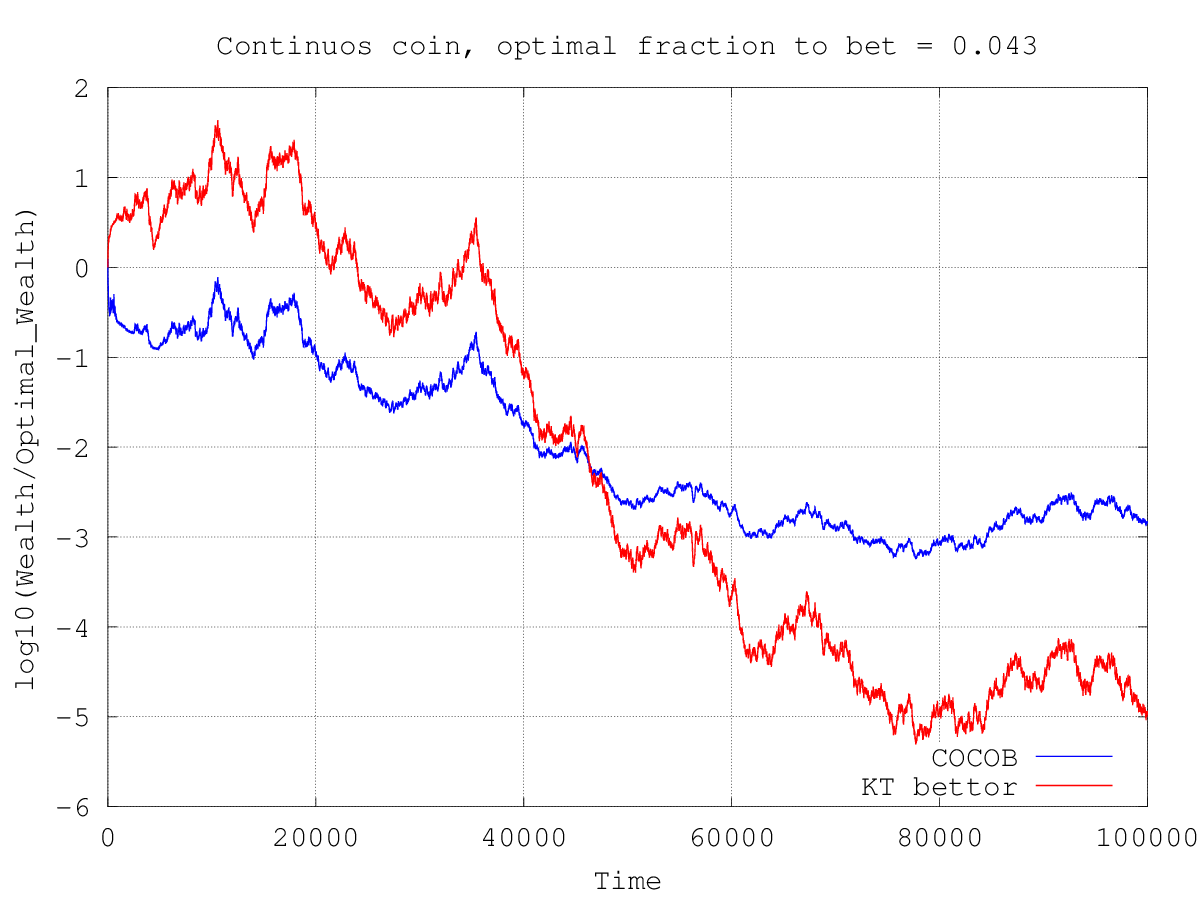
\includegraphics[width=0.45\linewidth]{code/continuos_coin.png}
\end{tabular}
\caption{Log ratio between the algorithms and the optimal a-posteriori fixed betting strategy, binary (left) and continuos (right) coin.}
\label{fig:bin_cont_coin}
\end{figure}

In this section we show some empirical results.

First, we tested the binary and continuos betting scenario. We compared the performance of \ac{COCOB} and the \ac{KT} algorithm, compared to the optimal a-posteriori fixed betting strategy. This latter one is simply computed as
\[
\beta^*=\argmax_{\beta} \ \prod_{t=1}^n (1+g_t \beta)~.
\]

In Figure~\ref{fig:bin_cont_coin}, we show the log ratio between the algorithms and the optimal a-posteriori fixed betting strategy. We see that, according to the theory, the performance of the \ac{KT} strategy on binary coin is better than the one of \ac{COCOB}. Also, the \ac{KT} algorithm is actually better than the a-posteriori fixed optimal strategy, because it adapts to small asymmetries at the beginning of the sequence of outcomes, resulting in a small fixed gain w.r.t. the fixed optimal strategy.

The situation is reversed in the more interesting setting of the continuos coin. Here, we see that \ac{COCOB} shows and advantage of \ac{KT}. Even more importantly, the difference between \ac{KT} and the optimal strategy sharply increases over time, due to the suboptimal nature of the \ac{KT} algorithm in this setting.